\documentclass[10pt, titlepage, german, a4paper]{article}
\usepackage[utf8]{inputenc}
\usepackage[T1]{fontenc}
\usepackage{lmodern}
%\usepackage{fixltx2e}
\usepackage{graphicx}
\usepackage{longtable}
\usepackage{float}
\usepackage{bigfoot}
%\usepackage{wrapfig}
\usepackage{rotating}
%\usepackage[normalem]{ulem}
\usepackage{amsmath}
\usepackage{textcomp}
%\usepackage{marvosym}
%\usepackage{wasysym}
\usepackage{amssymb}
\usepackage[hidelinks]{hyperref}
\tolerance=1000
\usepackage[normalem]{ulem}
\usepackage[ngerman, germanb]{babel}
%\usepackage{csquotes}
%\usepackage[square,sort,comma,numbers]{natbib}
\usepackage[style=alphabetic,sortlocale=de_DE,url=false,natbib=true,backend=bibtex]{biblatex}

%\usepackage{showkeys}
\usepackage{xpatch}

% patch macro used in bibliography
%\xpretobibmacro{bib+doi+url}
%{\iffieldundef{doi}
%	{}
%	{\clearfield{url}}}
%{}{}
\setlength{\parindent}{0cm}
%\usepackage[section]{placeins}
\usepackage{fancyhdr}
%\usepackage{subfig}
\usepackage{xcolor}
\usepackage{url}
%\usepackage[backend=biber,style=ieee,sortlocale=de_DE,
%url=false,doi=true,eprint=false]{biblatex}
\usepackage{standalone}
\usepackage{array,multirow,multicol}
%\usepackage{enumerate}
\usepackage{enumitem}
%\usepackage{tikz}
%\usepackage{tkz-berge}
%\usetikzlibrary{arrows, petri, topaths}
\usepackage{titlesec}
\usepackage{listings}
\usepackage{verbatim}
\titleformat{\section}[block]
{\fontsize{12}{15}\bfseries\rmfamily\filcenter}
{\thesection}
{1em}
{\MakeUppercase}
\titleformat{\subsection}[block]
{\fontsize{12}{15}\bfseries\rmfamily}
{\thesubsection}
{1em}
{}
\titleformat{\subsubsection}[block]
{\bfseries\rmfamily}
{\thesubsubsection}
{1em}
{}
\addbibresource{bibliography.bib}
\newcommand{\sectionbreak}{\clearpage}
\renewcommand{\lstlistingname}{Codeausschnitt}% Listing -> Algorithm

%\let\OLDitemize\itemize
%\renewcommand\itemize{\OLDitemize\addtolength{\itemsep}{-5pt}}

% TitelSeite
\renewcommand\maketitle{\begin{titlepage}%
    \singlespacing
    \begin{center}
      
      \hrule
      \vspace{1cm}
      \LARGE {\bf \sf Entwicklung von 3D-Darstellungen mit der HoloLens zur Unterstützung der Vermittlung physikalischer Inhalte}
      \vspace{1cm}
      \hrule
      
      \vspace{0.8cm}
      \Large {Masterarbeit}\\
      \vspace{1.0cm}
      \Large {Universität Rostock\\
	Fakultät für Informatik und Elektrotechnik\\
	Institut für Informatik}\\
      
      \vspace{1.2cm}
      
\includegraphics[width=2.34in]{include/unilogo.jpg}
      \vspace{1.0cm}
      
    \end{center}
    
    \Large
    \begin{tabular}{lcl}
      vorgelegt von: &&  Matthias Kuhr\\
      Matrikelnummer: && 212207426\\
      geboren am: && 07.04.1993 in Rostock\\
      Erstgutachter: && Prof. Dr. Heidrun Schumann\\
      Zweitgutachter: && Prof. Dr. Oliver Staadt\\
      Betreuer: && Dr. Christian Tominski\\
      Abgabedatum: && \today
    \end{tabular}
    \normalsize
    \clearpage
    % Selbstaendigkeitserklaerung
    \onehalfspacing
    \thispagestyle{empty}
    \section*{Selbstständigkeitserklärung}
    \vspace{2cm}

	Hiermit erkläre ich, Matthias Kuhr, dass ich die vorliegende schriftliche Masterarbeit selbst angefertigt und keine anderen als die angegebenen Hilfsmittel genutzt habe. % Alle Stellen, die wortwörtlich oder dem Sinn nach aus anderen Publikationen entnommen sind, habe ich klar gekennzeichnet und die Quelle angegeben. % An Stellen, die auf einen Zusammenarbeit mit anderen beruhen, habe ich deutlich gemacht, worin meine eigene Leistung besteht.
	
	%selbstständig und ohne unerlaubte fremde Hilfe angefertigt, keine anderen als die angegebenen Quellen und Hilfsmittel verwendet und die den verwendeten Quellen und Hilfsmitteln wörtlich oder inhaltlich entnommenen Stellen als solche kenntlich gemacht habe.
    \vspace{2cm}
    \begin{flushright}
      Rostock, den \today
    \end{flushright}

  \end{titlepage}%
}
\pagenumbering{roman}
\usepackage{setspace}
\onehalfspacing
\author{Matthias Kuhr}
\date{Entwurf vom \today}
\title{Entwicklung von 3D-Darstellungen mit der HoloLens zur Unterstützung der Vermittlung physikalischer Inhalte}

\begin{document}
	\maketitle
	\section*{Zusammenfassung}
Augmented Reality (AR) hat in den letzten Jahren durch die Verfügbarkeit entsprechender Hard- und Software an Bedeutung gewonnen. Darunter ist auch die HoloLens zu nennen, ein Head Mounted Display, das virtuelle Objekte in die Realität einbetten und anzeigen kann. Ein wichtiges Anwendungsfeld für AR-Anwendungen ist der Ausbildungsbereich und auch in der physikalischen Ausbildung wurde AR bereits erfolgreich eingesetzt. Auf Basis der HoloLens existieren jedoch kaum Arbeiten. Diese Arbeit untersucht daher den Einsatz des Gerätes im Kontext eines physikalischen Experimentes.\\
\noindent\hspace*{5mm}
Es wird eine Lösung vorgestellt, die einen Versuch mit einer Helmholtz-Spule durch eine AR-Anwendung erweitert und dabei Rücksicht auf die besonderen technischen Eigenschaften der HoloLens nimmt. Anhand von Positions- und Echtzeitdaten wird eine Magnetfelddarstellung in den Versuchsaufbau eingebettet. Außerdem werden theoretische Ergebnisse und zusätzliche Informationen (z.B. Stromrichtung) angezeigt. Dadurch werden andernfalls nicht sichtbarer physikalische Eigenschaften und Zusammenhänge für den Nutzer sichtbar.\\
\noindent\hspace*{5mm}
Gleichzeitig vermeidet die Lösung Probleme durch die Technik des Gerätes. Die Hologramme weisen eine gute Stabilität auf, liegen in einer geeigneten Entfernung und werden durch das begrenzte Field of View der HoloLens kaum beeinträchtigt. In ersten Reaktionen bewerteten Nutzer die Erfahrung durchgehend positiv. Die Ergebnisse motivieren eine Ausweitung und Übertragung des Ansatzes auf weitere Inhalte und Anwendungsfälle sowie eine empirische Evaluation der Ergebnisse.

%\section*{Abstract}
%In recent years augmented reality (AR) has risen in 
	\tableofcontents
	\clearpage
	%\bibliographystyle{alphadin}
	\newcounter{savepage}
	\setcounter{savepage}{\arabic{page}}
	\pagenumbering{arabic}
	\section{Einleitung}
\label{sec-1}
Augmented Reality (AR) hat in den letzten Jahren immer mehr an Bedeutung gewonnen. Nicht zuletzt durch Fortschritte im Bereich der künstlichen Intelligenz und immer leistungsfähiger werdender Hardware eröffnen sich neue Möglichkeiten, um die Realität digital zu erweitern und durch virtuelle Objekte anzureichern. Ein Gerät, mit dem solche Anwendungen möglich sind, ist die 2015 durch Microsoft vorgestellte HoloLens. Dabei handelt es sich um ein wie eine Brille getragenes Device, das in der Lage ist, virtuelle Objekte in der Umgebung des Nutzers zu platzieren und anzuzeigen. Das geschieht, indem die Objekte über transparente Displays in das Sichtfeld des Nutzers projiziert werden. Dabei wird der Nutzer nicht von seiner Umgebung isoliert, sondern kann diese weiterhin wahrnehmen.\\

Ein wichtiger Anwendungsbereich für AR-Technologie sind Ausbildung und Training. Daher gibt es in der Forschung ein zunehmendes Maß an Untersuchungen zum Einsatz von Augmented Reality in diesen Bereichen \cite{Bacca14}. Die Forschungen zeigen meist positive Auswirkungen auf die Lernleistung und Motivation durch AR-gestützte Lernanwendungen. Auch in der Physik 

Physikalische Experimente durch virtuelle Darstellungen anzureichern und so besser und intuitiver verständlich zu machen, ist kein völlig neuer Ansatz. So stellen Strzys et. al. eine Anwendung mit der HoloLens im Bereich der Thermodynamik vor, bei der das gemessene Wärmeprofil eines erhitzten Metallstabes virtuell mit Hilfe der HoloLens auf den Stab gelegt wird \cite{Strzys17}. Und Buchau et. al. präsentieren eine Lösung, die unter anderem das Magnetfeld zweier Helmholtz-Spulen in das Echtzeitbild der Webcam zeichnet \cite{Buchau09}.\\

\cite{Amiraslanov18}.  \cite{Javaheri18}

Motivation z.B. Einbinden von Informationen zu Versuchsaufbau, Visualisierung nicht sichtbarer physikalischer Größen und Vorgänge z.B. Magnetfeld und Stromfluss

%Augmenting Microsoft's HoloLens with vuforia tracking for neuronavigation \cite{Frantz18}
%HoloMuse: Enhancing Engagement with Archaeological Artifacts Through Gesture-Based Interaction with Holograms \cite{Pollalis17}

%HoloCPR: Designing and Evaluating a Mixed Reality Interface for Time-Critical Emergencies \cite{Johnson18}

\subsection{Fragestellung und prinzipieller Lösungsansatz}
\label{sec-1-2}
Die HoloLens ist ein AR-Device mit eigenen technischen Eigenschaften und Einschränkungen, die Auswirkungen darauf haben, ob und wie das Gerät in verschiedenen Anwendungsszenarien genutzt werden kann. Zum Einsatz im Bereich der Physik finden sich in der gängigen Literatur nur wenige Beispiele. Wie die Brille in der physikalischen Ausbildung dabei unterstützen kann, Konzepte und Zusammenhänge zu vermitteln, ist daher eine interessante Fragestellung. Die vorliegende Arbeit dringt in das Gebiet vor, indem sich näher mit der Unterstützung von Laborversuchen durch die HoloLens befasst wird. Dies geschieht anhand eines konkreten Beispiels: Die experimentelle Messung des Erdmagnetfeldes mit Hilfe einer Helmholtz-Spule.\\

Die konkrete Fragestellung dieser Arbeit lautet daher:
\begin{center}
	\textit{\textbf{Wie kann die HoloLens in dem konkreten Anwendungsfall eines physikalischen Versuches genutzt werden?}}
\end{center}

Es wird untersucht, mit welchen virtuellen Elementen der Versuch durch die HoloLens angereichert werden kann und wie diese Integration erfolgt. Der Lösungsansatz basiert darauf, die technischen Möglichkeiten der AR-Technologie zu nutzen, um nicht direkt sichtbare physikalische Eigenschaften in ihrem realen Kontext anzuzeigen und durch eine räumliche und zeitliche Einbettung in Zusammenhang zum Versuchsaufbau zu setzen. Gleichzeitig werden jedoch technische Limitierungen berücksichtigt, um negative Auswirkungen auf die Nutzererfahrung zu vermeiden. Ziel ist es, eine AR-Lösung mit der HoloLens zu entwickeln, die auf der einen Seite wichtige physikalische Eigenschaften und Zusammenhänge sichtbar und erfahrbar macht, und auf der anderen Seite eine komfortable Nutzung ermöglicht.

\begin{comment}
\subsection{Aufgabenstellung}

Im Rahmen der Arbeit soll anhand der HoloLens untersucht werden, wie diese in der Physik-Lehre eingesetzt werden kann, um physikalische Inhalte zu vermitteln. Insbesondere soll betrachtet werden, wie physikalische Experimente mittels Mixed Reality Anwendungen durch zusätzliche Inhalte angereichert werden können.\\

\par
Dazu sind zunächst die technischen Möglichkeiten und Voraussetzungen der HoloLens zu betrachten und in Zusammenhang mit dem Anwendungsfall zu bringen. Weiterhin sind bestehende Ansätze im Einsatz von Mixed Reality Technologie in der Lehre, besonders in der Physik-Lehre, herauszuarbeiten und einzuordnen.

Davon ausgehend soll der Fragestellung anhand eines konkreten Beispiels nachgegangen werden. Für einen ausgewählten Versuchsaufbau sind die darzustellenden Objekte und Informationen sowie das Zusammenspiel dieser mit dem aufgebauten Experiment, der Umgebung und den Nutzern zu entwickeln. Für den ausgewählten Anwendungsfall soll eine Umsetzung mit der HoloLens konzipiert, designet und prototypisch implementiert werden.
\end{comment}

\subsection{Aufbau der Arbeit}
\label{sec-1-3}
Die vorliegende Arbeit ist wie folgt aufgebaut. Kapitel \ref{sec-2} erläutert notwendige Hintergrundinformationen zur Technik der HoloLens, deren Anwendung in der Lehre sowie die physikalischen Hintergründe des Versuches. Kapitel \ref{sec-3} kristallisiert die Anforderungen für den konkreten Anwendungsfall heraus und präzisiert die Problemstellung. In Abschnitt \ref{sec-4} werden die gewählten Lösungsansätze vorgestellt, deren Implementierung in Kapitel \ref{sec-5} erörtert wird. Kapitel \ref{sec-6} stellt die Ergebnisse heraus und diskutiert diese im Rahmen der Fragestellung. Abschließend fasst Kapitel \ref{sec-7} die Ergebnisse zusammen und gibt einen Ausblick.
	\section{Hintergrund}
\label{sec-2}

	\section{Hintergrund}
\label{sec-2}

Die Arbeit baut auf bestehende Erkenntnisse aus drei Bereichen auf. Ausgangspunkt ist die HoloLens mit ihrem technischen Hintergrund. Daraus ergeben sich für diese Arbeit technische Anforderungen und Einschränkungen, die es zu berücksichtigen gilt. Daher wird die Technik mit ihren Implikationen in Kap. \ref{sec-2-1} vorgestellt.\\

Außerdem fußt die Arbeit auf bestehenden Erkenntnissen und Ansätzen aus der Lehre, insbesondere im Bereich der Physik. Aufgrund der Aktualität der HoloLens existieren hier zum Zeitpunkt dieser Arbeit nur begrenzt Arbeiten auf Basis des Gerätes. Gleichzeitig existieren bereits ähnliche Ansätze zur der Anwendung von Augmented Reality in der Physik mit anderen Geräten. Deshalb wird auf Forschungsergebnisse aus dem weiteren Bereich des Einsatzes von Augmented Reality zurückgegriffen, die in Kap. \ref{sec-2-2} erörtert werden.\\

Auf Basis der beiden vorangegangenen Abschnitte motiviert schließlich Kap. \ref{sec-2-3} den gewählten physikalischen Versuch und erläutert dazu notwendige Hintergrundinformationen.

\subsection{HoloLens}
\label{sec-2-1}
Die HoloLens ist ein von Microsoft entwickeltes \textit{Head-Mounted Display} (HMD), das seit 2016 auf dem Markt ist. Das Gerät ist in der Lage, virtuelle Darstellungen in der Umgebung des Trägers zu verankern und anzuzeigen. Anders als bei anderen Geräten wird dabei die Umgebung nicht durch eine Kamera wahrgenommen wie z.B. bei einer Anwendung mit einem Smartphone, sondern direkt mittels durchsichtiger Displays. Einen Eindruck von dem Gerät vermittelt Abbildung \ref{img:hololens}. Bevor näher auf die technischen Eigenschaften dieser Lösung eingegangen wird, soll zunächst eine kurze Einordnung der Gerätes erfolgen.

\subsubsection{Einordnung der HoloLens}
\label{sec-2-1-1}
TODO Problem Mixed Reality vs Augmented Reality auflösen

\begin{figure}[h!]
	\centering
	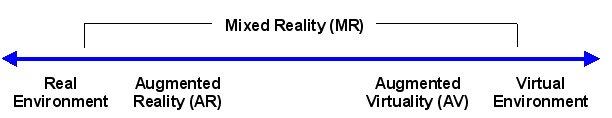
\includegraphics[width=0.9\textwidth]{images/papers/virtual_continuum.png}
	\caption{Virtual Continuum eingeführt von Paul Milgram \cite{Milgram94}}
	\label{img:virtual_continuum}
\end{figure}

Der Begriff \textit{Mixed Reality} (MR) wurde von Paul Milgram und Fumio Kishino in deren Arbeit \textit{``A Taxonomy of Mixed Reality Visual Displays''} im Jahr 1994 eingeführt \cite{Milgram94}. Die Autoren stellen das Konzept eines \textit{Virtual Continuums} vor, einem kontinuierlichen Spektrum zwischen vollständig realer und vollständig virtueller Umgebung. Augmented Reality findet sich damit auf der linken Seite des Spektrums wieder, dem entgegen steht Augmented Virtuality auf der rechten Seite. Als Mixed Reality wird der gesamte Bereich des Continuums bezeichnet, der zwischen den beiden Extremen ``völlig real'' und ``völlig virtuell'' liegt. Schema \ref{img:virtual_continuum} skizziert diesen Zusammenhang.\\

\begin{comment}
An dieser Stelle sei erwähnt, dass sich auch andere Interpretationen des MR-Begriffes finden. So beschreibt Jon Peddie MR als Kombination von realer und virtueller Welt, bei der beide co-existieren, wobei die MR Anwendung Informationen über die Umgebung und darin vorhandene Objekte nutzt \cite{Peddie17}. MR wird also eher als Erweiterung von AR verstanden, als eine übergeordnete Kategorie. Diese Herangehensweise findet sich auch bei manchen Internetquellen\footnote{https://www.intel.de/content/www/de/de/tech-tips-and-tricks/virtual-reality-vs-augmented-reality.html} \footnote{https://www.forbes.com/sites/quora/2018/02/02/the-difference-between-virtual-reality-augmented-reality-and-mixed-reality}.\\
\end{comment}

Beim Begriff der \textit{Augmented Reality} (AR), der ebenfalls kurz definiert werden soll, folgt diese Arbeit der gängigen Definition von Ronald T. Azuma \cite{Azuma97}. Dabei werden unter AR Techniken zusammengefasst, die es dem Nutzer erlauben, die reale Welt zu sehen, welche überlagerte oder eingebettete virtuelle Objekte enthält. Dafür hat eine Technik drei Charakteristiken aufzuweisen, sie:
\begin{enumerate}
	\setlength{\itemsep}{-5pt}
	\item Kombiniert reales und virtuelles
	\item Ist interaktiv (in Echtzeit)
	\item Steht in einem dreidimensionalen, räumlichen Zusammenhang
\end{enumerate}

\begin{comment}
Entsprechend der zuvor angesprochenen Variationen im Verständnis von Mixed Reality gibt es Diskussionen darüber, wie die HoloLens zu klassifizieren ist. Microsoft selbst ordnet sie als MR Gerät ein. Andere argumentieren, die Möglichkeiten der Brille seinen mit dem Begriff der Augmented Reality bereits abgedeckt. Peddie beispielsweise schreibt, dass ``Microsoft jedoch, möglicherweise aus Gründen des Marketing und der besseren Produktabgrenzung, darauf besteht, sie sei als MR Device einzuordnen'' \footnote{Zitat frei aus dem Englischen übersetzt.} \cite{Peddie17}.\\

Da diese Arbeit sich am MR Begriff von Milgram orientiert und mit der HoloLens unterschiedlich stark immersive Anwendungen möglich sich, wird die HoloLens im Folgenden allgemein als MR Device bezeichnet.
\end{comment}

Die HoloLens deckt mit ihren technischen Möglichkeiten vor allem den linken Bereich des Spektrums ab. Viele Anwendungen liegen deshalb im Teilbereich Augmented Reality. Die technischen Eigenschaften und genutzten Techniken des HMDs bringen verschiedene Implikationen und Einschränkungen für Anwendungen auf der HoloLens mit sich. Daher soll nun auf die technischen Aspekte näher eingegangen werden.\\

\begin{figure}[h!]
	\centering
	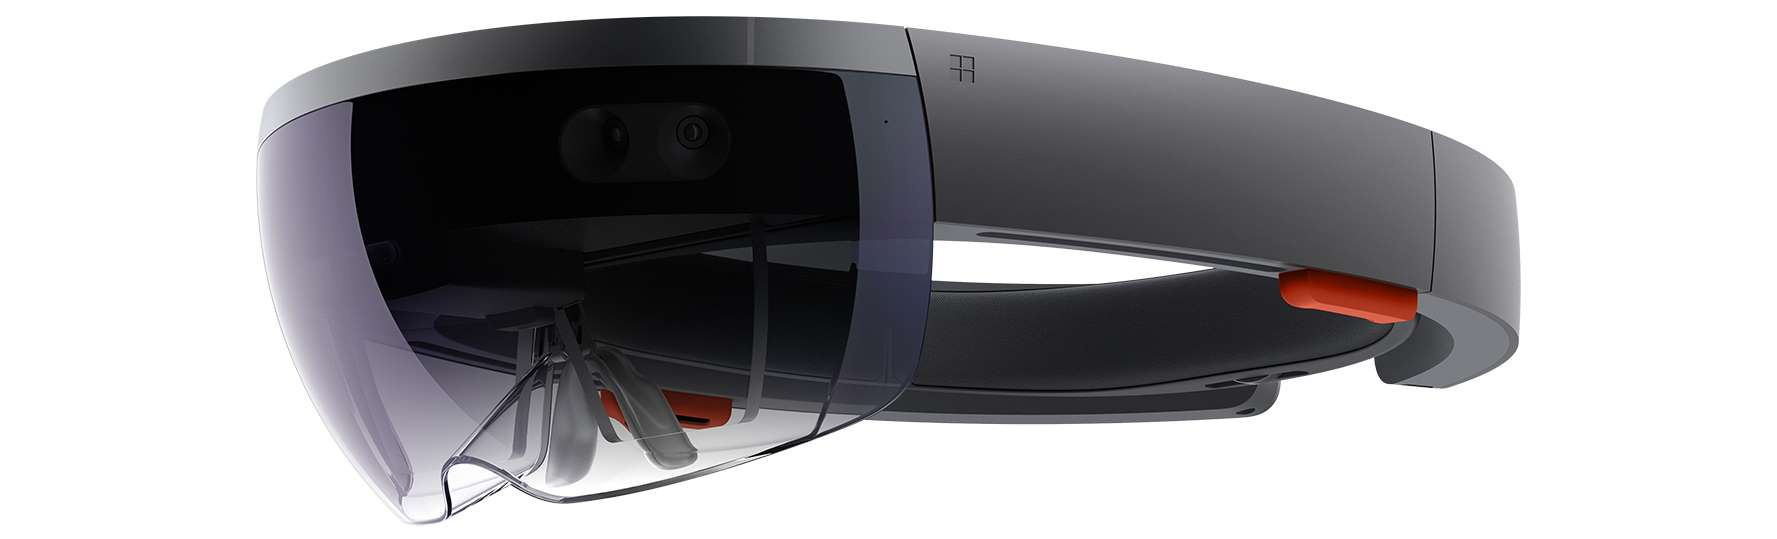
\includegraphics[width=0.9\textwidth]{images/papers/hololens.jpg}
	\caption{Die HoloLens in der Developer Edition (Quelle: Microsoft)}
	%https://www.microsoft.com/de-de/hololens
	\label{img:hololens}
\end{figure}

\subsubsection{Die Hardware}
\label{sec-2-1-2}
Bei dem Device handelt es sich um einen eigenständigen Computer, auf dem eine spezielle Version von Windows 10 läuft. Die Brille arbeitet also völlig autonom und ist nicht auf externe Hardware wie z.B. zusätzliche Rechen- und Batterieeinheiten angewiesen.\\

\vspace{4px}
\textit{Das Display}\\
Kernstück des Gerätes ist das durchsichtige, stereoskopische Display, mit dem die virtuellen 3D-Objekte angezeigt werden. Durchsichtig bedeutet, dass das Display für Licht von außen durchlässig ist und der Nutzer somit wie durch eine Brille seine Umgebung sehen kann. Virtuelle Objekte werden zusätzlich dazu angezeigt, indem Licht über optische Wellenleiter (Optical Wave Guides) in das Display geleitet wird, welches das Licht dann auf die Augen reflektiert.\\

Anwendungen werden mit 60 Frames pro Sekunde dargestellt. Bei der Anzeige handelt es sich jedoch um ein \textit{Color Sequential Display}, bei dem die drei Farben Rot, Grün und Blau nacheinander dargestellt werden. Pro Bild werden folglich drei Einzelbilder (je eins pro Farbe) gezeigt, was eine Framerate von 240 Hz ergibt.\\

Es handelt sich dabei um ein stereoskopisches Display, bei dem pro Auge separat ein Bild dargestellt wird. So ermöglicht die HoloLens dem Träger das stereoskopische Wahrnehmen dreidimensionaler Objekte. Die beiden Bilder werden in einem festen Abstand von 22 mm zueinander dargestellt. Außerdem beträgt die Distanz, auf die sich die Augen einstellen müssen, damit Bilder als scharf wahrgenommen werden (Akkommodation), etwa zwei Meter und ist ebenfalls fest.\\

\vspace{4px}
\textit{Das Tracking}\\
Um die Hologramme im Raum verankern zu können, benötigt die HoloLens Informationen über ihre exakte Position und Orientierung im Raum. Beides erarbeitet das Gerät allein aus einem Zusammenspiel der verschiedenen internen Sensoren und ist nicht auf externe Markierungen angewiesen, es handelt sich um sogenanntes \textit{Inside-Out Tracking}. Das Vorgehen basiert dabei auf zwei Strategien.
\par
\noindent\hspace*{5mm}
Zum einen erfasst die HoloLens die Oberflächenstruktur der Umgebung über Tiefen- und Stereokameras. Während der Nutzer sich durch den Raum bewegt, wird dies immer weiter vervollständigt und verbessert. Dieses Vorgehen wird \textit{Spatial Mapping} genannt und kann auch von Anwendungen genutzt werden, um mit Objekten der realen Welt zu interagieren. Eine Darstellung der optischen Sensoren ist in Abb. \ref{img:hololens_tech} enthalten.
\par
\noindent\hspace*{5mm}
Zum anderen kommt eine inertiale Messeinheit zum Einsatz. Über die Beschleunigungs-, Rotations- und Magnetflusssensoren können Änderungen in Position und Ausrichtung der Brille gemessen werden. Bei diesem Vorgehen summieren sich Messfehler im Laufe der Zeit jedoch stetig weiter auf und die Positionsschätzung wird zunehmend unzuverlässiger. Daher wird ein Zusammenspiel mit der Raumerkennung genutzt.


\begin{figure}[h!]
	\centering
	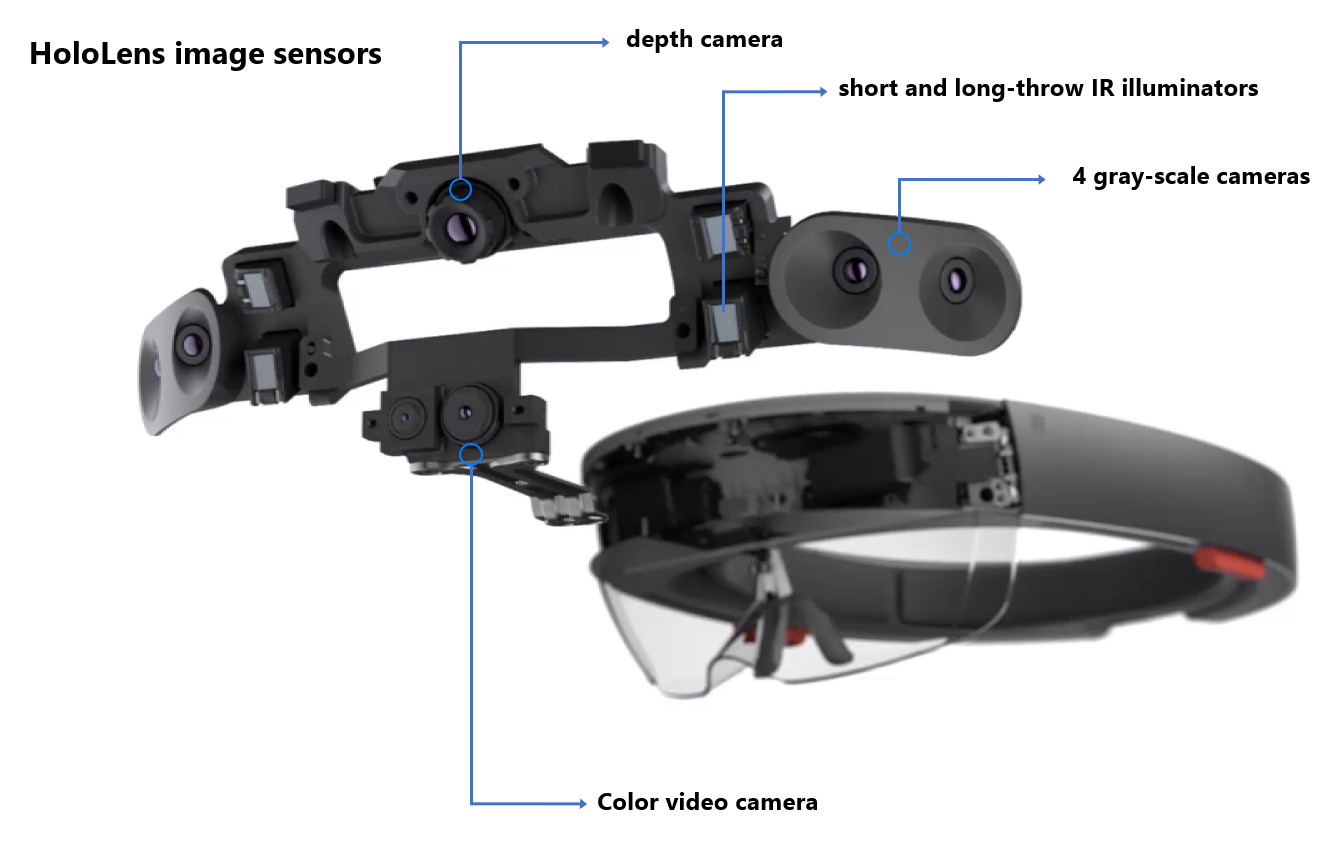
\includegraphics[width=0.9\textwidth]{images/papers/hololens_tech.png}
	\caption{Überblick über die optischen Sensoren der HoloLens \cite{MRDoc}}
	%https://docs.microsoft.com/en-us/windows/mixed-reality/hololens-hardware-details
	\label{img:hololens_tech}
\end{figure}

Einen Überblick über die verwendete Hardware gibt Tabelle \ref{tab:hololens_tech_details}.

\bgroup
\setlength\extrarowheight{0pt}
\def\arraystretch{1.25}
\begin{table}[h!]
	\centering
	\begin{tabular}{l|l}
		Kategorie & Eigenschaft\\
		\hline
		\hline
		Anzeige & 1268 x 720 Pixel pro Auge\\
		& 60 Hz Bildwiederholrate\\
		& Blickfeld ca. 34° (diagonal), 16:9 Format\\
		\hline
		Prozessor & Intel 32-Bit Prozessor @ 1.0 GHz\\
		\hline
		Grafik & Microsoft Holographic Processing Unit (HPU)\\
		\hline
		Arbeitsspeicher & 2 GB RAM\\
		& 1 GB HPU RAM\\
		\hline
		Speicher & 64 GB Flash Speicher\\
		\hline
		Kamera & 2 MP Foto / HD Video Front-Kamera\\
		\hline
		Sensoren & Inertiale Messeinheit (Accelerometer, Gyroskop, Magnetometer) \\
		& Zwei Stereo Kameras\\
		& 120° x 120° Tiefenkamera\\
		& Vier Mikrofone\\
		& Ambient Light Sensor\\
		\hline
		Akku & 2-3h Akkulaufzeit \\
		\hline
		Gewicht & 579 Gramm \\
		\hline
		Konnektivität & WiFi, BLE, USB 2.0, 3.5 mm Audio Jack \\
		\hline
		Audio & Lautsprecher mit Raumklang-Unterstützung\\
		\hline
		Steuerung & Gestensteuerung\\
		& Sprachsteuerung\\
		& HoloLens Klicker, Controller, Maus, Tastatur\\
	\end{tabular}\caption{\label{tab:hololens_tech_details} Technische Spezifikation der HoloLens \cite{MRDoc}.}
\end{table}
\egroup

\subsubsection{Die Software und Interaktion}
\label{sec-2-1-3}
Auf der HoloLens läuft eine spezielle Version von Windows 10. Diese benötigt weniger Resourcen im Vergleich zu einem herkömmlichen PC und hat daher auch einen eingeschränkten Funktionsumfang. Anwendungen werden in Form von UWP Apps bereitgestellt. Hier unterstützt Microsoft die Entwicklung mit Unity und stellt entsprechende Toolkits zur Verfügung.\\

Die Steuerung durch den Nutzer erfolgt auf vier verschiedene Arten:
\begin{itemize}[topsep=-2px]
	\setlength{\itemsep}{-1pt}
	\singlespacing
	\item Blickrichtung (Orientierung des Kopfes)
	\item Handgesten
	\item Sprachbefehle
	\item Externe Eingabegeräte (Controller, Maus, Tastatur, etc.)
\end{itemize}
\vspace{6px}

Handgesten werden von der HoloLens automatisch erkannt und an die Anwendung in Form von Events weitergegeben, auf welche dann reagiert werden kann. Hier sind aktuell verschiedene Klick-Gesten zu nennen, durch die bekannte Mausfunktionen wie Klick, Click-and-Hold, Doppelklick und Drag-and-Drop abgebildet werden. Der Cursor orientiert sich dabei an der aktuellen Blickrichtung: Es wird automatisch das Objekt angeklickt, das als erstes von einer zentralen, vorwärts gerichteten Linie getroffen würde. Außerdem gibt es eine spezifische Handgeste zum aufrufen des Hauptmenüs.\\

Darüber hinaus nimmt die HoloLens englische Wörter als Sprachbefehle an, die sich auch kombinieren lassen. So kann eine Anwendung die Phrase ''Hello World'' als Keyword registrieren und dann darauf reagieren. Über Bluetooth lassen sich weitere Eingabegeräte anschließen: Den mit der HoloLens mitgelieferten Klicker, der die Klick-Geste ersetzen kann, aber auch eine Tastatur oder ein Controller lassen sich nutzen.\\

\vspace{4px}
\textit{Das Mixed Reality Toolkit}\\
Das \textit{Mixed Reality Toolkit} (MRTK) ist ein quelloffenes Toolkit, das elementare Funktionen für die Entwicklung von Mixed Reality Anwendungen, insbesondere auch für die HoloLens, bereitstellt. Dazu gehört beispielsweise ein Objekt, das den zuvor genannten Cursor implementiert, aber auch Funktionen, die das Spatial Mapping auswerten. Für die Entwicklung mit Unity gibt es das Toolkit als Unitypackage, das unter anderem folgende Features bereitstellt:

\begin{itemize}[topsep=-2px]
	\setlength{\itemsep}{-1pt}
	\singlespacing
	\item Kameraobjekt mit den korrekten Einstellungen für die HoloLens
	\item Stabilisiertes Cursorobjekt mit Animationen für verschiedene Klicks
	\item Manager-Objekte, die Steuerung von Inputs und des Spatial Mappings erlauben
	\item Skripte für Standard Interaktionen wie Drag-and-Drop und Skalierung
	\item Für HoloLens angepasste Materialien und Shader
	\item Vorgefertigte und anpassbare UI-Elemente wie Buttons, Tooltips, Icons und Dialoge
\end{itemize}
\vspace{6px}

Für die Entwicklung mit dem Toolkit und der HoloLens existiert ein umfassendes Repertoire aus Dokumentation, Beispielen, Guidelines, Einführungen und Hinweisen.\\


\subsubsection{Implikationen für Anwendungsdesign}
\label{sec-2-1-4}
Die technischen Eigenschaften der HoloLens haben Auswirkung auf Design und Nutzung von Anwendungen. Dazu gehören auch technisch bedingte Einschränkungen sowie zu berücksichtigende Aspekte für die Usability und Nutzererfahrung. Im Folgenden soll auf ausgewählte solcher Zusammenhänge hingewiesen werden.\\

\textit{Tracking}\\
Ein wichtiger Punkt ist, das Tracking nicht zu behindern, da die Darstellungen andernfalls nicht korrekt im Raum positioniert werden können. Für die Stereo- und Tiefenkamera sind sehr dunkle und transparente Materialien problematisch, da hier kaum (Infrarot-) Licht reflektiert wird und so entsprechende Gegenstände nicht erkannt werden. Spiegelnde Materialien sind daher ebenfalls ungünstig.\\

\textit{Display}\\
Die Displays sind, vergleichbar mit einem Beamer, in der Lage den Hintergrund zu überblenden, nicht jedoch ihn abzudunkeln. Dementsprechend ist kein Schwarz darstellbar. Wie transparent Objekte auf der HoloLens erscheinen, hängt folglich auch vom Hintergrund und der Umgebungshelligkeit ab. Ein sehr heller Hintergrund kann von der HoloLens nicht vollständig überblendet werden.
\par
\noindent\hspace*{5mm}
Außerdem hängt die Transparenz virtueller Objekten von ihrer Farbe ab. Ein blauer Pixel leuchtet nur in jedem dritten Frame auf, ein weißer hingegen in jedem Frame, da die Farben sequentiell dargestellt werden.\\

Bedingt durch die Displaytechnik wirken Objekte scharf, wenn sich die Augen auf eine Distanz von zwei Metern einstellen (Akkommodation). Die Augen sind jedoch daran gewöhnt, dass nah liegende Objekte eine andere Akkommodation erfordern, als weiter entfernte. Dies kann vor allem bei sehr dicht liegenden Objekten dazu führen, dass Nutzer sich unwohl fühlen oder die Objekte nicht richtig erkennen können.

\begin{minipage}{0.48\textwidth}
	\centering
	\includegraphics[width=0.9\textwidth]{images/todo.jpg}
	\label{img:acco-convergence}
\end{minipage}\begin{minipage}{0.48\textwidth}
	\centering
	\includegraphics[width=0.9\textwidth]{images/todo.jpg}
\end{minipage}\\

\par
\noindent\hspace*{5mm}
Im Zusammenhang der Akkommodation spielt hier auch die Konvergenz der Augen eine Rolle. Darunter versteht man die Bewegung der Augen aufeinander zu, sodass der Punkt, in dem sich die Gesichtslinien treffen, näher kommt. Eine Illustration des Zusammenhangs bietet Abbildung \ref{img:acco-convergence}. Dieser Vorgang ist wichtig, damit Objekte nicht doppelt gesehen werden. Akkommodation und Konvergenz sind auf natürliche Weise gekoppelt: Um ein dicht liegendes Objekt zu betrachten laufen die Augen weiter zusammen und erhöhen ihre Brechkraft. Dieser Effekt wird auch Akkommodation-Konvergenz-Reflex genannt. Beim Tragen der HoloLens kann es jedoch dazu kommen, dass dieses Zusammenspiel aufgebrochen wird.
\par
\noindent\hspace*{5mm}
Angenommen ein Nutzer fokussiert ein reales Objekt in einer Entfernung unter zwei Metern. Jetzt wird ein virtuelles Objekt räumlich vor dem realen Objekt positioniert. Jetzt müssen Akkommodation und Konvergenz gegenläufig arbeiten: Die Augen müssen sich aufeinander zu bewegen, die Brechkraft dabei jedoch abnehmen, da sie sich auf zwei Meter anpassen muss. Dies steht im Gegensatz zum Akkommodation-Konvergenz-Reflex und kann die Nutzererfahrung negativ beeinflussen.\\

Sowohl für Akkommodation als auch Konvergenz gilt jedoch, dass die Unterschiede mit zunehmender Distanz kleiner werden und die Probleme deshalb vor allem bei kurzen Distanzen auftreten.\\

\textit{Hardwareressourcen}\\
Die Hardwareressourcen der HoloLens sind mit einer CPU und GPU mit jeweils 1 GHz und 1GB RAM stark limitiert. Anwendungen sollten daher möglichst ressourcenschonend sein. Auf rechenintensive Operationen wie z.B. Schattenberechnungen oder Kantenglättung muss meist verzichtet werden.\\

\textit{Framerate}\\
Dabei ist es von besonderer Bedeutung, dass die Anwendung möglichst konstant 60 Bilder pro Sekunde ausgibt. Um die Hologramme im Raum stabil und ohne Ruckler oder Zittern anzuzeigen, müssen selbst feinste Kopfbewegungen ausgeglichen werden. Dazu nutzt die HoloLens ein spezielles Verfahren:
\par
\noindent\hspace*{5mm}
Bevor eine Szene in die Render-Pipeline geht, trifft die Brille anhand der Sensordaten eine Vorhersage darüber, in welcher Position und Ausrichtung sich die Brille befinden wird, wenn das zu errechnende Bild dargestellt wird. Anhand dieser Schätzung wird die Kamera-Position und -Ausrichtung für die Szene festgelegt und anschließend gerendert. Eine längere oder variierende Renderzeit bedeutet damit auch eine unzuverlässigere Schätzung. Das kann zu instabil wirkenden Darstellungen führen, z.B. in Form von Zittern oder Ruckeln. Deshalb empfiehlt Microsoft, die Framerate von 60 FPS stets aufrecht zu erhalten.

\subsubsection{Empfehlungen zu Design und Umsetzung}
\label{sec-2-1-5}
Damit Einschränkungen umgangen und negative Auswirkungen vermieden werden können, gibt es bereits einige Designempfehlungen und Guide-Lines sowie Empfehlungen zur Implementierung. Die Dokumentation zu Windows Mixed Reality umfasst hier einige Kriterien, Vorschläge und Hinweise, von denen besonders relevante hier vorgestellt werden sollen.\\

\textit{Qualitätskriterien}\\
Als Referenz dafür, wie gut eine Anwendung technische Einschränkungen berücksichtigt, kann eine Liste von Qualitätskriterien dienen, anhand derer Anwendungen bewertet werden können \cite{MRDocQuality}. Diese deckt viele der zuvor erläuterten Probleme wie z.B. der Abstand zu Objekten ab. Jedes Kriterium ist mit einer Beschreibung versehen, unter welchen Umständen es als optimal erfüllt, erfüllt oder nicht erfüllt gilt. Eine Kurzfassung relevanter Kriterien ist in Tabelle \ref{tab:tech_criteria} zusammengestellt.\\
\bgroup
\setlength\extrarowheight{-2pt}
\def\arraystretch{1.8}
\begin{table}[H]
	\centering
	\begin{tabular}{m{2.3cm}|m{8.5cm}}
		Kriterium & Kurzbeschreibung \\
		\hline
		\hline
		Framerate & Gibt die Anwendung konstant 60 FPS aus?\\
		\hline
		Stabilität der Hologramme & Weisen Hologramme bei Bewegungen Ruckler, Sprünge, Drift, Wackeln, Wippen oder ähnliches auf?\\
		\hline
		Positionierung & Sind Hologramme im Verhältnis zu realen Objekten korrekt positioniert?\\
		\hline
		Komfortzone & Liegen Distanz und Betrachtungswinkel in den empfohlenen Bereichen?\\
		\hline
		Tiefen Wechsel & Bedingt die Anwendung häufige Fokuswechsel?\\
		\hline
		FOV-Grenzen & Beeinträchtigen die Begrenzungen des FOV die Nutzererfahrungen?\\
		\hline
		Input Interaction Clarity & Werden konsistente, bekannte und geeignete Eingabemethoden geboten?\\
		\hline
		Anpassung an Nutzerposition & Passen sich Darstellungen der Position des Nutzers an?\\
		\hline
		Interaktive Objekte & Sind interaktive Objekte als solche erkennbar?\\
		\hline
		Ladevorgänge  & Erhält der Nutzer Feedback über länger laufende Operationen?\\
	\end{tabular}\caption{\label{tab:tech_criteria} Kurzfassung der Qualitätskriterien. Eine ausführliche Version mit genauen Kriterien und Methoden zur Evaluierung findet sich in \cite{MRDocQuality}.}
\end{table}
\egroup

\textbf{Positionierung von Objekten}\\
Zur Anordnung von Objekten gibt es einige Design-Guidelines, von denen ausgewählte hier genannt werden sollen. Die Dokumentation nennt die Folgenden Richtlinien:
\begin{itemize}
	\setlength{\itemsep}{-1pt}
	\singlespacing
	\item Distanz zur Kamera optimal bei 2m, Komfortzone 1-5m, Blickwinkel zwischen 0° und 35°
	\item Größe für interaktive Objekte min. 1,5° - 3° Grad in der Vertikalen
	\item Positionierung möglichst nah an Spatial Anchors und der Stabilization Plane
\end{itemize}

\textit{Distanz}\\
Objekte sollten typischerweise aus einer Distanz zwischen einem und fünf Metern betrachtet werden, um die zuvor erläuterten Probleme mit der Wahrnehmung zu vermeiden. Deshalb sollten Objekte ausgeblendet werden, die zu nah kommen. Neben der Distanz spielt auch der Blickwinkel in der vertikalen eine Rolle. Damit ein Anwender die Darstellungen angenehm betrachten kann ist es wichtig, eine angenehme und natürliche Kopfposition zu ermöglichen. Hier wird ein Blickwinkel zwischen 0° und 35° unterhalb der Horizontlinie empfohlen.\\

\textit{Größe}\\
Weiterhin ist die Größe von Objekten von Bedeutung. Das gilt besonders dann, wenn sie mit dem an die Kopfbewegungen gekoppelten Cursor anvisiert werden müssen. Zu kleine Objekte wären für den Anwender schwer zu treffen. Ein Winkel zwischen 1,5° und 3° des Sichtfeldes dienen hier als Orientierung. Allerdings sollten die Darstellungen auch nicht zu groß sein, da sie sonst schon bei geringen Kopfbewegungen durch die Begrenzung des Displays abgeschnitten werden.\\

Um Objekte wie z.B. Menus und Dialoge, die nicht fest im Raum verankert sind, anzupassen, stellt das Mixed Reality Toolkit verschiedene Funktionen wie z.B. Billboarding oder Tagalong zur Verfügung, die Abstand, Orientierung und Skalierung entsprechend der Nutzerbewegung automatisch anpassen.\\

\textit{Stabilisierung}\\
Die HoloLens maximiert die Stabilität von Hologrammen gegen eine ausgewählte Ebene, die von der Anwendung selbst dynamisch gesetzt werden kann. Hologramme sollten daher, sofern sie gerade betrachtet werden, möglichst nah an dieser Ebene liegen, um stabil zu wirken.\\

\textit{Performance Optimierungen}\\
Da die Framerate maßgeblichen Einfluss auf die Stabilität von Hologrammen hat und die Hardwareressourcen limitiert sind, gibt es eine Reihe von empfohlenen Optimierungen und Hinweisen, um die Performance einer Anwendung zu verbessern. Diese umfassen unter anderem:
\begin{itemize}[topsep=-2px]
	\setlength{\itemsep}{-1pt}
	\singlespacing
	\item Singe Pass Instanced Rendering verwenden
	\item Z-Puffer Größe auf 16 Bit setzen
	\item Full-Screen Post Processing (z.B. FXAA) vermeiden
	\item Shader anpassen / vereinfachen
	\item Physics ausschalten
	\item Overdraw reduzieren
\end{itemize}
\vspace{6px}

Um die Performance bei der Entwicklung im Blick haben zu können gibt es einige Tools. Die HoloLens stellt über ein Webinterface einen Performance-Monitor zur Verfügung. Dieser gibt Auskunft über die Auslastung von Ressourcen wie CPU und GPU, ähnlich zum Windows Taskmanager. Außerdem verfügt Unity über einen Profiler, der detailliertere Informationen zum Renderingprozess liefert.\\

\textit{Weitere Empfehlungen}\\
Aus ihren Erfahrungen und dem Nutzerfeedback aus mehreren HoloLens-Applikationen geben Zimmer et. al. einige weitere Empfehlungen \cite{Zimmer17}. Im Folgenden ist eine Auswahl an für diese Arbeit besonders relevanten Aspekten zusammengefasst:
\begin{itemize}[topsep=-2px]
	\setlength{\itemsep}{-1pt}
	\singlespacing
	\item Einen sichtbaren Cursor in der Mitte des Blickfeldes für die Auswahl bzw. das Anklicken von Objekten nutzen
	\item Begrenzungen des Field-of-View (FOV) beachten: Wenn möglich Objektegröße so anpassen, dass diese ganz dargestellt werden können, da andernfalls Objekte weniger präsent wirken
	\item Die Einbettung von Objekten kann durch visuelle Anhaltspunkte wie Verdeckung oder Schatten unterstützt werden
	\item Spatial Mesh für grobe Verdeckung nutzbar, für genauere Verdeckung können reale Objekte nachmodelliert werden 
	\item Alternative Interaktionsmöglichkeiten (z.B. Klicker) können hilfreich sein, wenn Nutzer Probleme mit Gesten oder der Sprachsteuerung haben
	\item Eine Einführung in die Anwendung und insbesondere die Steuerung kann hilfreich sein, da der Umgang mit der HoloLens oder ähnlichen Geräten für Anwender meist ungewohnt ist
\end{itemize}
\vspace{6px}


	\subsection{Auswahl des Experimentes und physikalischer Hintergrund}
\label{sec-2-3}
Welches Experiment unterstützt und welche physikalischen Zusammenhänge damit vermittelt werden sollen, bestimmt die inhaltlichen Aspekte einer Lösung. 

Helmholtz-Spulen werden in der Physik an verschiedenen Stellen verwendet und spielen auch in der Ausbildung von Schülern und Studenten eine wichtige Rolle. Unter anderem werden sie in Schülerversuchen genutzt, um experimentell die Stärke des Erdmagnetfeldes zu bestimmen. Im Folgenden sollen die physikalischen Hintergründe kurz eingeführt sowie der Versuchsaufbau und -Ablauf erläutert werden.

Zuvor soll jedoch kurz auf die Auswahl des vorgestellten Versuches eingegangen werden.

\subsubsection{Auswahl des Experimentes}
\label{sec-2-3-1}
Das Experiment wurde aus mehreren Gründen für diese Arbeit ausgewählt. Zum einen ist Augmented Reality für die Darstellung von Magnetfeldern eine bekannte Methode. Bestehende Arbeiten auf dem Gebiet motivieren den Einsatz der Technik in diesem Kontext. Aus dieser Perspektive ist das Experiment mit der Helmholtz-Spule geeignet, da die entstehenden Magnetfelder dabei im Fokus stehen. Außerdem bietet der Anwendungsfall Potential zur Erweiterung auf andere Experimente mit einer Helmholtz-Spule. Aber auch weitere, teilweise komplexere Inhalte wie z.B. das Biot-Savart-Gesetz ließen sich daran anknüpfen.\\

Neben diesen Motivationen wurde der Versuch auch aus technischen und praktischen Aspekten ausgewählt. Im Wesentlichen trugen dazu die folgenden Faktoren bei:
\begin{itemize}
	\singlespacing
	\item Das Magnetfeld der Spule hat keine erkennbaren Auswirkungen auf die HoloLens (das Gerät nutzt ein Magnetometer). Tests im Vorfeld mit Flussdichten von über 100 Mikrotesla zeigten keine wahrnehmbaren Auswirkungen auf das Tracking und die Stabilität von Hologrammen
	\item Die notwendigen Materialien (Spule, Messgeräte, Simulationslösung) standen für diese Arbeit zur Verfügung
	\item Die gegebene Größe der Spule (R=15cm) eignet sich für das beschränkte Sichtfeld der HoloLens.
	\item Das Experiment enthält keine sich schnell bewegenden Elemente und ist bis auf den Kompass statisch, es erfordert außerdem keine besondere Schutzausrüstung
	\item Der physikalische Hintergrund des Versuches nicht so komplex, als dass eine Auseinandersetzung damit den Rahmen dieser Arbeit sprengen würde
\end{itemize}

Einige dieser Umstände begünstigen einen Einsatz der Brille für diesen konkreten Anwendungsfall und sind ggf. bei anderen Szenarien so nicht gegeben.\\

\subsubsection{Spulen und Magnetfelder}
\label{sec-2-3-2}
Ein Magnetfeld kann als dreidimensionales Vektorfeld aufgefasst werden. Die Stärke an einem Punkt lässt sich über den Feldstärkevektor $\boldsymbol{H}$ sowie die Flussdichte $\boldsymbol{B}$ angeben. Beide Größen hängen über eine Materialkonstante $\mu$ zusammen: $\boldsymbol{B} = \mu \cdot \boldsymbol{H}$.
\par
\noindent\hspace*{5mm}
Wird eine Leiterschleife von einem elektrischen Strom durchflossen, so induziert diese ein Magnetfeld. Dieses Feld verläuft sowohl durch das Innere als auch durch die Umgebung der Spule. Die Stärke des Feldes hängt dabei von der Windungszahl und dem Durchmesser der Spule sowie der anliegenden Stromstärke ab.
Im Zentrum der Spule ist das Magnetfeld \textit{homogen}. Das bedeutet, es ist an allen Punkten im Raum gleich stark und gleich gerichtet. Außerhalb und am Rand der Spule hingegen ist das Feld \textit{inhomogen}, es erfüllt beide zuvor genannten Eigenschaften nicht.\\

\textit{Darstellungsformen von Magnetfeldern}\\
Zur Visualisierung von Magnetfeldern gibt es unterschiedliche Darstellungsmodelle. Im Bereich der Lehre haben sich davon vor allem zwei etabliert: Feldlinien und Vektoren. Beide stellen das Feld mit Richtung und Stärke im Raum dar, unterscheiden sich aber in der Art und Weise. Abbildung \ref{img:Magnetfeld-Helmholtzspule} zeigt eine gemeinsame Darstellung beider Ansätze für eine Helmholtz-Spule.\\

\begin{figure}[h!]
	\centering
	\includegraphics[width=0.65\textwidth]{images/papers/Magnetfeld-Helmholtzspule.jpg}
	\caption{Magnetfeld einer Helmholtz-Spule in der X-Z-Ebene \cite{wiki:15}. Der Betrag der Vektoren wurde hier statt der Länge über die Farbe kodiert. Die Feldlinien sind für einen mittigen Ausschnitt der Spule gezeichnet. Im Inneren ist das Feld weitgehend homogen.} %\footnote{\url{https://de.wikipedia.org/wiki/Helmholtz-Spule}}}
	\label{img:Magnetfeld-Helmholtzspule}
\end{figure}

\textit{Das Feldlinienmodell}\\
Die Feldliniendarstellung ist wohl die häufiger anzutreffende Darstellungsform. Hier werden kontinuierliche Linien genutzt, um den magnetischen Fluss darzustellen. Die Richtung des Feldstärkevektors an einem Punkt auf einer Feldlinie entspricht der Tangente an diesem Punkt. Die Stärke des Feldes wird meist proportional zur Dichte der Feldlinien dargestellt \cite{Kilian03}.\\

Diese Darstellung macht den Unterschied zwischen homogenen und inhomogenen Feldern besonders gut sichtbar, da bei einem homogenen Feld die Feldlinien parallel verlaufen, bei einem inhomogenen hingegen nicht. Außerdem ist die Darstellung über die Dichte der Feldlinien eng verbunden mit dem Konzept des magnetischen Flusses.\\

Allerdings bedeutet diese Darstellungsform auch, dass um so stärker das Feld ist, desto mehr Feldlinien auf gleichem Raum dargestellt werden müssen. Außerdem ist bei sich ändernden Feldern schwer zu erkennen, ob sich nur die Beträge der Feldstärkevektoren ändern, oder auch deren Richtungen. Denn in beiden Fällen verändern sich Form und Abstand der Feldlinien.\\

\textit{Vektorfeld}\\
Im Gegensatz dazu wird in der Vektor-Darstellung das Feld über einzelne Vektoren repräsentiert. Dabei geben Richtung und Betrag eines Vektors den Feldstärkevektor des Magnetfeldes für genau einen Punkt an.\\
So lässt sich die Feldstärke an einem durch einen Vektor repräsentierten Punkt im Raum direkt ablesen. Wo ein Feld homogen ist lässt sich jedoch nur durch das Vergleichen von mehreren Vektoren in Länge und Richtung feststellen. Dieses Modell hat gegenüber dem Feldlinienmodell jedoch den Vorteil, dass mit zunehmender Feldstärke die Vektoren nur länger werden, ihre Anzahl jedoch gleich bleibt. Außerdem ist hier klar zu erkennen, ob bei einem sich ändernden Feld die Richtung der Vektoren konstant bleibt, oder nicht.

\subsubsection{Helmholtz-Spule}
\label{sec-2-3-3}
Bei einer Helmholtz-Spule handelt es sich im Prinzip um zum zwei zusammengeschaltete solcher Spulen. Dabei werden zwei identische Spulen nebeneinander aufgestellt und verbunden, sodass der Abstand genau dem Radius der Spulen entspricht. Abbildung \ref{img:Helmholtz} zeigt eine solche Helmholtz-Spule.\\
\begin{wrapfigure}{R}{0.4\textwidth}
	\centering
	\includegraphics[width=0.38\textwidth]{images/papers/Helmholtz.jpg}
	\caption{Foto der verwendeten Helmholtz-Spule. Radius und Abstand betragen 15 cm und jede Teilspule hat 124 Windungen \cite{3BS}.}
	\label{img:Helmholtz}
\end{wrapfigure}


Durch diese spezielle Eigenschaft des Aufbaus überlagern sich die beiden, durch die einzelnen Spulen entstehenden Magnetfelder genau so, dass im Raum zwischen den Spulen ebenfalls ein (nahezu) homogenes Magnetfeld entsteht. Abbildung \ref{img:Magnetfeld-Helmholtzspule} zeigt das Feld für die X-Z-Ebene in der Draufsicht von oben auf eine Helmholtz-Spule. Dabei ist zu erkennen, dass das Feld in weiten Teilen des durch die zwei Spulen aufgespannten Zylinders homogen ist. Lediglich am Rand und in unmittelbarer Nähe zu den Spulen wird das Feld zunehmend inhomogen. Detailliertere Informationen dazu finden sich beispielsweise in \cite{Demtroder13}.\\

Das Feld wird durch elliptische Integrale beschrieben, die nur numerisch zu lösen sind.
Die magnetische Flussdichte einer Helmholtz-Spule im Mittelpunkt zwischen den Spulen vereinfacht sich jedoch zu folgender Gleichung:
\begin{equation}
\label{eq:mfield}
B = \mu_{0} \cdot \frac{8 \cdot I \cdot N}{\sqrt{125} \cdot R}
\end{equation}

Dabei entspricht $I$ der Stromstärke, $N$ der Anzahl Windungen, $R$ dem Radius und $\mu_{0}$ die magnetische Feldkonstante. Die Stromstärke tritt dabei in der Feldgleichung als linearer Faktor auf. Änderungen an der Stromstärke rufen eine dazu proportionale Änderung der Feldstärke hervor. Außerdem bedeutet dieser Umstand, dass die Richtung des Feldstärke- bzw. Flussdichtevektors nicht von der Stromstärke abhängt, sondern konstant bleibt.\\

\subsubsection{Versuchsaufbau und Ablauf}
\label{sec-2-3-4}
Ziel des Versuches ist die Bestimmung des Erdmagnetfeldes. Genauer bedeutet das die experimentelle Bestimmung von Richtung und magnetischer Flussdichte des Feldes. Die Richtung kann dabei allein über den Kompass bestimmt werden. Die Flussdichte wird mittels Gleichung \ref{eq:mfield} aus der gemessenen Stromstärke ermittelt, bei der die Helmholtz-Spule ein gleich starkes, eigenes Magnetfeld erzeugt.\\

\textit{Aufbau}\\
Der Versuchsaufbau ist in Abbildung \ref{img:experiment-devices} dargestellt und besteht aus: 
\begin{itemize}
	\setlength{\itemsep}{-5pt}
	\item Einer Helmholtz-Spule mit fester Windungszahl und festem Radius
	\item Einem mittig in der Spule positionierten Kompass
	\item Einem in Reihe geschalteten Amperemeter
	\item Einem in Reihe geschalteten Widerstand	
	\item Einer angeschlossenen Spannungsquelle
\end{itemize}

\begin{figure}[h!]
	\centering
	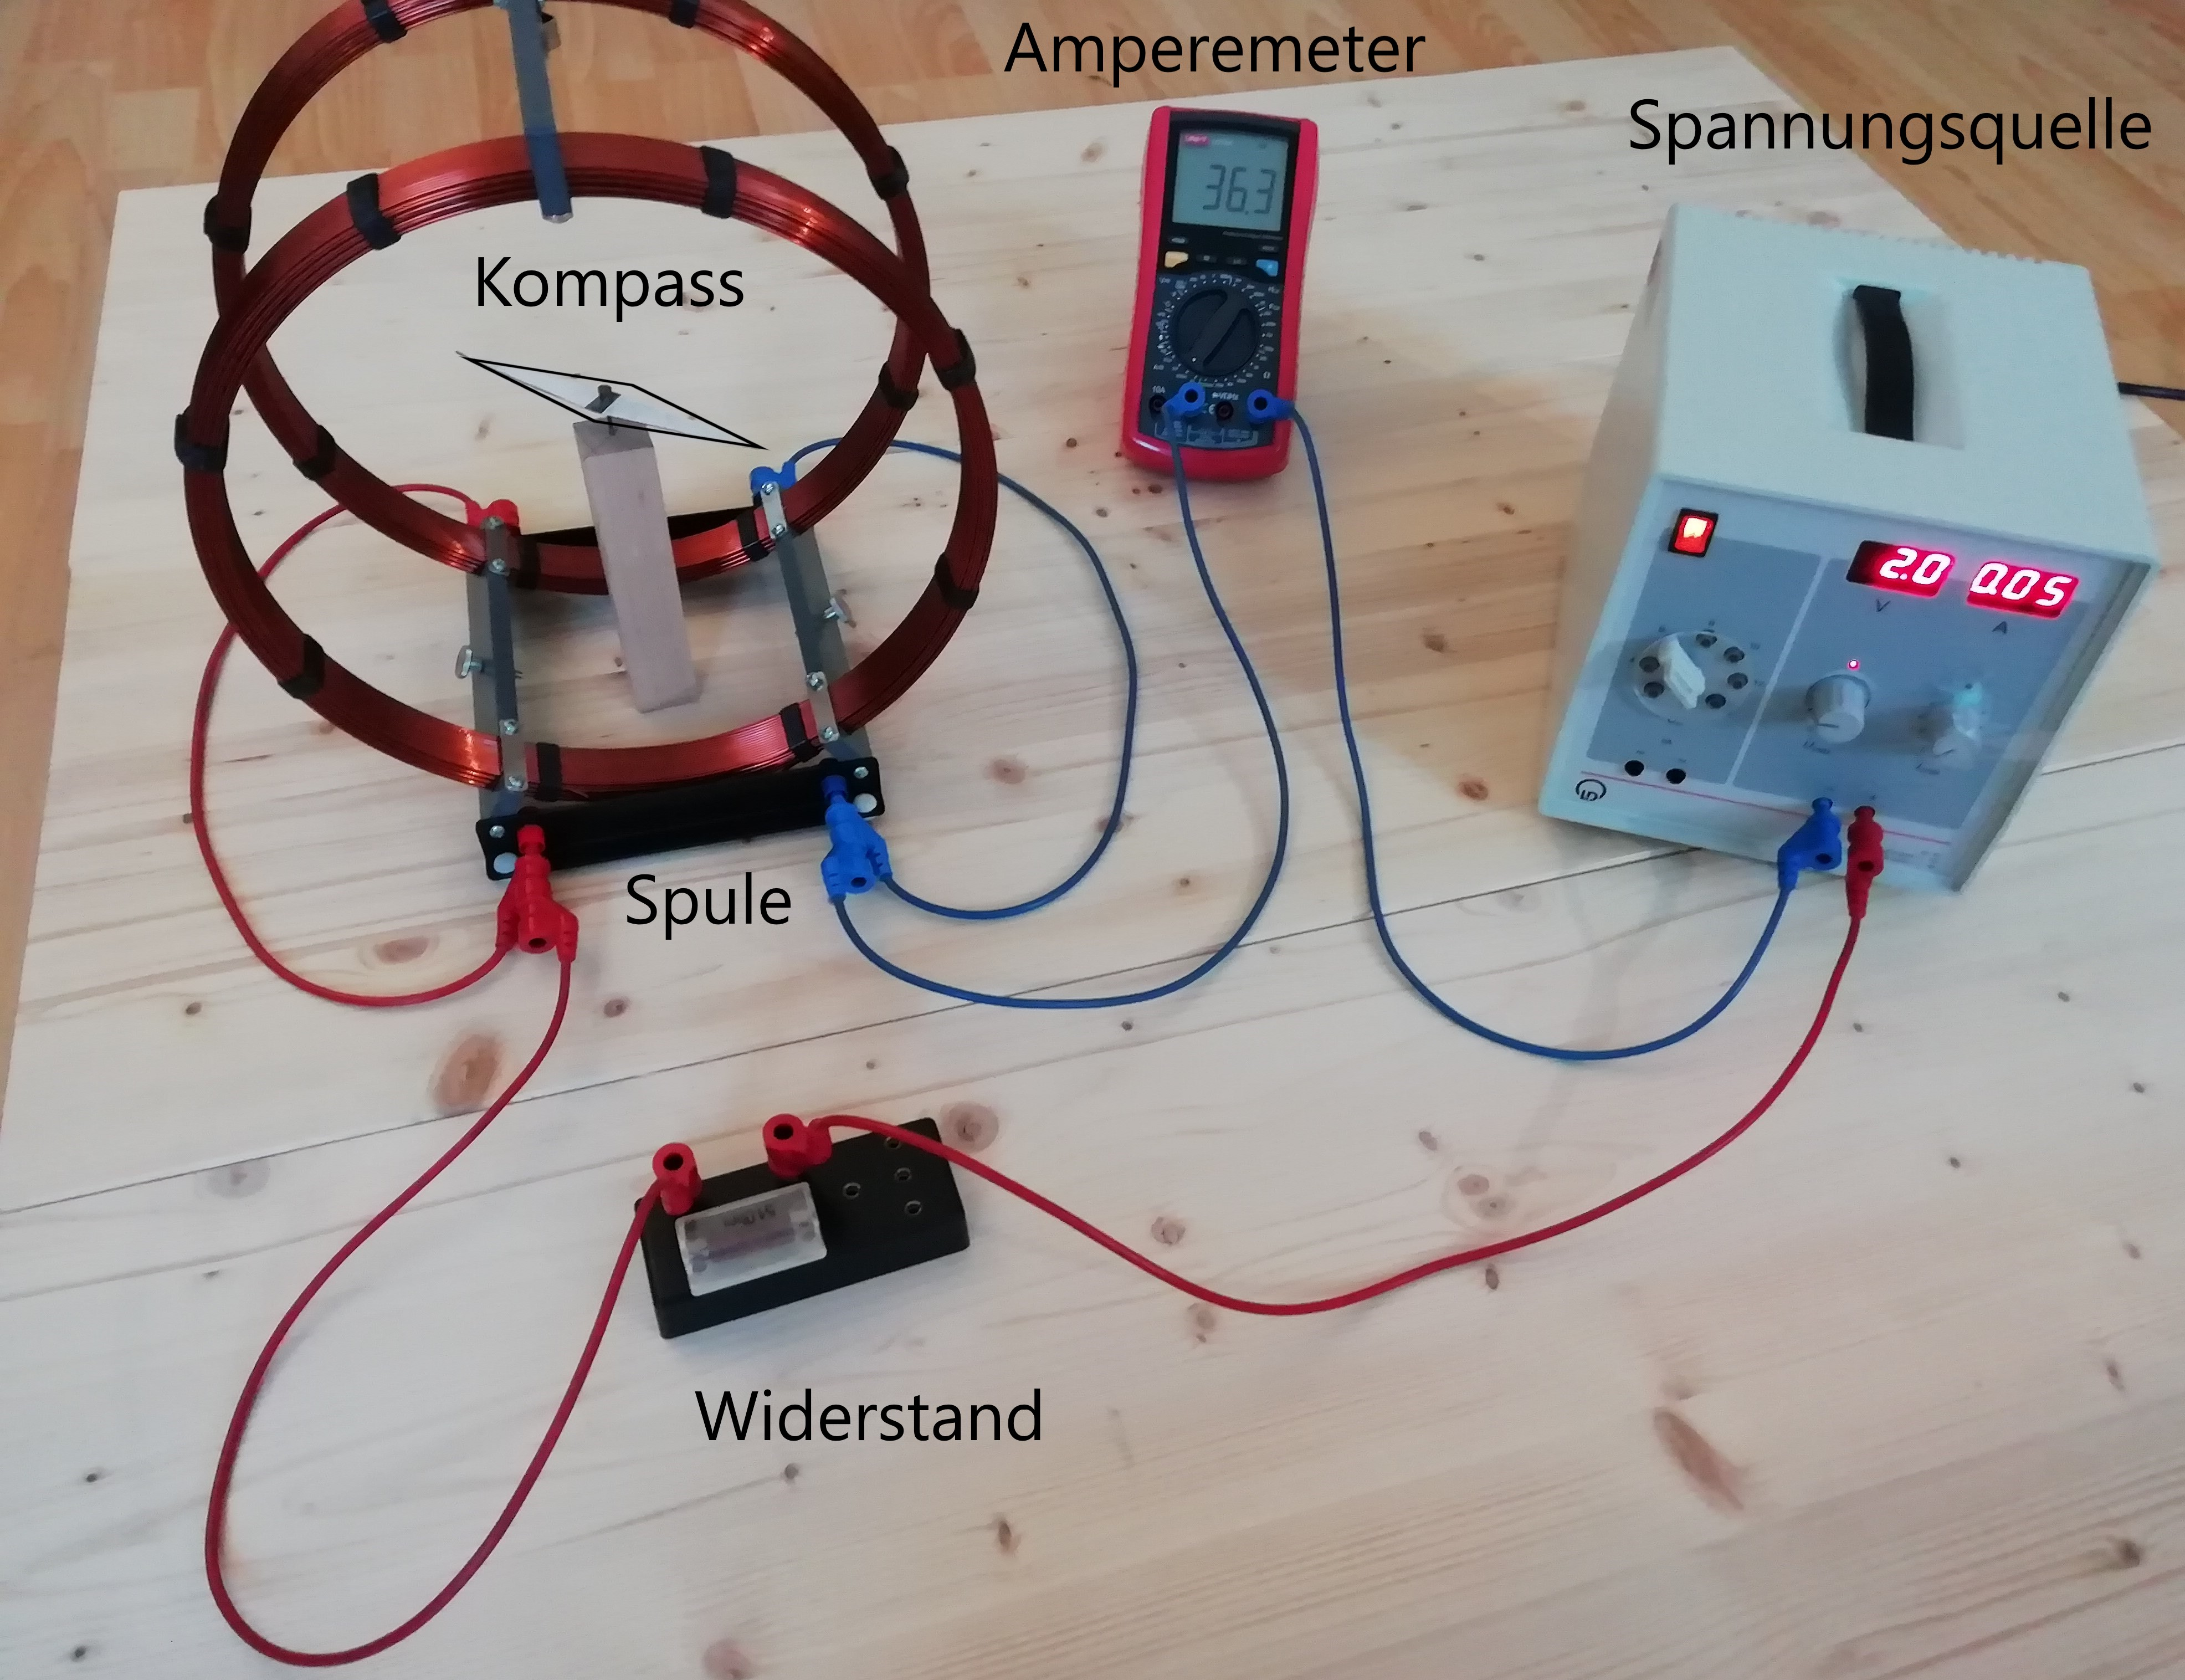
\includegraphics[width=0.8\textwidth]{images/papers/setup_labled.jpg}
	\caption{Foto des Versuchsaufbaus. Die Helmholt-Spule besteht aus zwei parallel geschalteten Spulen. Der Widerstand passt den Bereich der einstellbaren Stromstärke an. Der weiß überklebte Kompass wurde nachträglich schwarz umrandet, damit er auf dem Foto besser zu sehen ist.}
	\label{img:experiment-devices}
\end{figure}

\textit{Ablauf}\\
Der Versuch läuft in zwei Teilen ab. Zunächst wird die Ausrichtung des Erdmagnetfeldes bestimmt und im nächsten Schritt dann die Flussdichte. Der Ablauf lässt sich wie folgt zusammenfassen:
\begin{enumerate}
	\setlength{\itemsep}{-2pt}
	\item Kompassnadel nach Norden ausrichten lassen
	\item Helmholtz-Spule orthogonal zur Kompassnadel ausrichten
	\item Spannungsquelle einschalten und Spannung langsam erhöhen
	\item Spannung erhöhen, bis Kompassnadel um 45° ausgelenkt ist
	\item Stromstärke ablesen und in Gleichung \eqref{eq:mfield} einsetzen
\end{enumerate}

Durch dieses Vorgehen wird im zweiten Schritt durch die Spule ein Magnetfeld erzeugt, das orthogonal zu dem der Erde gerichtet ist. Beide Felder überlagern sich, so dass sie den Kompass genau dann gleichmäßig in beide Richtungen auslenken, wenn beide Felder gleich stark auf die Nadel wirken.


	\subsection{Physikalischer Hintergrund}
\label{sec-2-2}
\begin{comment}
\begin{center}
\fbox{
\parbox{0.9\linewidth}{
\textit{Ziel des Kapitels:}\\
Anwendungsfall und Hintergrund vorstellen.
}}\\
\end{center}
\end{comment}

Helmholtz-Spulen werden in der Physik an verschiedenen Stellen verwendet und spielen auch in der Ausbildung von Schülern und Studenten eine wichtige Rolle. Unter anderem werden sie in Schülerversuchen genutzt, um experimentell die Stärke des Erdmagnetfeldes zu bestimmen. Im Folgenden sollen die physikalischen Hintergründe kurz eingeführt sowie der Versuchsaufbau und -Ablauf erläutert werden.

\subsubsection{Spulen und Magnetfelder}
\label{sec-2-2-1}
Ein Magnetfeld kann als dreidimensionales Vektorfeld aufgefasst werden. Die Stärke an einem Punkt lässt sich über den Feldstärkevektor $\boldsymbol{H}$ sowie die Flussdichte $\boldsymbol{B}$ angeben. Beide Größen hängen über eine Materialkonstante $\mu$ zusammen: $\boldsymbol{B} = \mu \cdot \boldsymbol{H}$.
\par
\noindent\hspace*{5mm}
Wird eine elektrische Leiterschleife von einem Strom durchflossen, so induziert diese ein Magnetfeld. Dieses Feld verläuft sowohl durch das Innere als auch durch die Umgebung der Spule. Die Stärke des Feldes hängt dabei von der Windungszahl und dem Durchmesser der Spule sowie der anliegenden Stromstärke ab.
Im Zentrum der Spule ist das Magnetfeld \textit{homogen}. Das bedeutet, es ist an allen Punkten im Raum gleich stark und gleich gerichtet. Außerhalb und am Rand der Spule hingegen ist das Feld \textit{inhomogen}, es erfüllt beide zuvor genannten Eigenschaften nicht.\\

%\vspace{4px}
\textit{Darstellungsformen von Magnetfeldern}\\
Zur Visualisierung von Magnetfeldern gibt es unterschiedliche Darstellungsmodelle. Im Bereich der Lehre haben sich davon vor allem zwei etabliert: Feldlinien und Vektoren. Beide stellen das Feld mit Richtung und Stärke im Raum dar, unterscheiden sich aber in der Art und Weise. Abbildung \ref{img:Magnetfeld-Helmholtzspule} zeigt eine gemeinsame Darstellung beider Ansätze für eine Helmholtz-Spule.\\

\begin{figure}[h!]
	\centering
	\includegraphics[width=0.65\textwidth]{images/Magnetfeld-Helmholtzspule.jpg}
	\caption{Magnetfeld einer Helmholtz-Spule in der X-Z-Ebene. Der Betrag der Vektoren wurde hier statt der Länge über die Farbe kodiert. Die Feldlinien sind für einen mittigen Ausschnitt der Spule gezeichnet. Die Homogenität des Feldes im Inneren ist klar zu erkennen. Bildquelle: Wikipedia} %\footnote{\url{https://de.wikipedia.org/wiki/Helmholtz-Spule}}}
	\label{img:Magnetfeld-Helmholtzspule}
\end{figure}

\textit{Das Feldlinienmodell}\\
Die Feldliniendarstellung ist wohl die häufiger anzutreffende Darstellungsform. Hier werden kontinuierliche Linien genutzt, um den magnetischen Fluss darzustellen. Die Richtung des Feldstärkevektors an einem Punkt auf einer Feldlinie entspricht der Tangente an diesem Punkt. Die Stärke des Feldes wird meist proportional zur Dichte der Feldlinien dargestellt \cite{Kilian03}.\\

Diese Darstellung macht den Unterschied zwischen homogenen und inhomogenen Feldern besonders gut sichtbar, da bei einem homogenen Feld die Feldlinien parallel verlaufen, bei einem inhomogenen hingegen nicht. Außerdem ist die Darstellung über die Dichte der Feldlinien eng verbunden mit dem Konzept des magnetischen Flusses.\\

Allerdings bedeutet diese Darstellungsform auch, dass um so stärker das Feld ist, desto mehr Feldlinien auf gleichem Raum dargestellt werden müssen. Außerdem ist bei sich ändernden Feldern schwer zu erkennen, ob sich nur die Beträge der Feldstärkevektoren ändern, oder auch die Richtungen. Denn in beiden Fällen verändern sich Form und Abstand der Feldlinien.\\

\textit{Vektorfeld}\\
Im Gegensatz dazu wird in der Vektor-Darstellung das Feld über einzelne Vektoren repräsentiert. Dabei geben Richtung und Betrag eines Vektors den Feldstärkevektor des Magnetfeldes für genau einen Punkt an.\\
So lässt sich die Feldstärke an einem durch einen Vektor repräsentierten Punkt im Raum direkt ablesen. Wo ein Feld homogen ist lässt sich jedoch nur durch das Vergleichen von mehreren Vektoren in Länge und Richtung feststellen. Dieses Modell hat gegenüber dem Feldlinienmodell jedoch den Vorteil, dass mit zunehmender Feldstärke die Vektoren nur länger werden, ihre Anzahl jedoch gleich bleibt. Außerdem ist hier klar zu erkennen, ob bei einem sich ändernden Feld die Richtung der Vektoren konstant bleibt, oder nicht.

\subsubsection{Helmholtz-Spule}
\label{sec-2-2-2}
Bei einer Helmholtz-Spule handelt es sich im Prinzip um zum zwei zusammengeschaltete solcher Spulen. Dabei werden zwei identische Spulen nebeneinander aufgestellt und verbunden, sodass der Abstand genau dem Radius der Spulen entspricht. Abbildung \ref{img:Helmholtz} zeigt eine solche Helmholtz-Spule.\\

\begin{figure}[h!]
	\centering
	\includegraphics[width=0.45\textwidth]{images/Helmholtz.jpg}
	\caption{HH Spule}
	\label{img:Helmholtz}
\end{figure}

Durch diese spezielle Eigenschaft des Aufbaus überlagern sich die beiden, durch die einzelnen Spulen entstehenden Magnetfelder genau so, dass im Raum zwischen den Spulen ebenfalls ein (nahezu) homogenes Magnetfeld entsteht. Abbildung \ref{img:Magnetfeld-Helmholtzspule} zeigt das Feld für die X-Z-Ebene in der Draufsicht von oben auf eine Helmholtz-Spule. Dabei ist zu erkennen, dass das Feld in weiten Teilen des durch die zwei Spulen aufgespannten Zylinders homogen ist. Lediglich am Rand und in unmittelbarer Nähe zu den Spulen wird das Feld zunehmend inhomogen. Detailliertere Informationen dazu finden sich beispielsweise in \cite{Demtroder13}.\\

Das Feld wird durch elliptische Integrale beschrieben, die nur numerisch zu lösen sind.
Die magnetische Flussdichte einer Helmholtz-Spule im Mittelpunkt zwischen den Spulen vereinfacht sich jedoch zu folgender Gleichung:
\begin{equation}
	\label{eq:mfield}
	B = \mu_{0} \cdot \frac{8 \cdot I \cdot N}{\sqrt{125} \cdot R}
\end{equation}

Dabei entspricht $I$ der Stromstärke, $N$ der Anzahl Windungen, $R$ dem Radius und $\mu_{0}$ der magnetischen Permeabilität. Die Stromstärke tritt dabei in der Feldgleichung als linearer Faktor auf, Änderungen an der Stromstärke rufen eine dazu proportionale Änderung der Feldstärke hervor. Das bedeutet aber auch, dass die Richtung der Feldstärkevektoren nicht von der Stromstärke abhängt, sondern konstant bleibt. Mit einer Lösung der Feldgleichung für ausgewählte Punkte im Raum kann dementsprechend das Feld für jede beliebige anliegende Stromstärke in diesen Punkten dargestellt werden.\\

\subsubsection{Versuchsaufbau und Ablauf}
\label{sec-2-2-3}
Ziel des Versuches ist die Bestimmung des Erdmagnetfeldes. Genauer bedeutet das die experimentelle Bestimmung von Richtung und magnetischer Flussdichte des Feldes. Die Richtung kann dabei allein über den Kompass bestimmt werden. Die Flussdichte wird aus der gemessenen Stromstärke ermittelt, bei der die Helmholtz-Spule ein gleich starkes, eigenes Magnetfeld erzeugt.\\

\textit{Aufbau}\\
Der Versuchsaufbau ist in Abbildung \ref{img:experiment-devices} dargestellt und besteht aus: 
\begin{itemize}
	\setlength{\itemsep}{-5pt}
	\item Einer Helmholtz-Spule mit fester Windungszahl und festem Radius
	\item Einem Kompass
	\item Einem in Reihe geschalteten Amperemeter
	\item Einer angeschlossenen Spannungsquelle
\end{itemize}

\begin{figure}[h!]
	\centering
	\includegraphics[width=0.8\textwidth]{images/todo.jpg}
	\caption{Versuchsaufbau}
	\label{img:experiment-devices}
\end{figure}

\textit{Ablauf}\\
Der Versuch läuft in zwei Teilen ab. Zunächst wird die Ausrichtung des Erdmagnetfeldes bestimmt und im nächsten Schritt dann die Flussdichte. Der Ablauf lässt sich wie folgt zusammenfassen:
\begin{enumerate}
	\setlength{\itemsep}{-2pt}
	\item Kompassnadel nach Norden ausrichten lassen
	\item Helmholtz-Spule orthogonal zur Kompassnadel ausrichten
	\item Spannungsquelle einschalten und Spannung langsam erhöhen
	\item Spannung erhöhen, bis Kompassnadel um 45° ausgelenkt ist
	\item Stromstärke ablesen und in Gleichung \eqref{eq:mfield} einsetzen
\end{enumerate}

Durch dieses Vorgehen wird im zweiten Schritt durch die Spule ein Magnetfeld erzeugt, das orthogonal zu dem der Erde gerichtet ist. Beide Felder überlagern sich, so dass sie den Kompass genau dann gleichmäßig in beide Richtungen auslenken, wenn beide Felder gleich stark auf die Nadel wirken.
	
	\section{Problemstellung und Requirements}
\label{sec-3}
\fbox{
	\parbox{\linewidth}{
		\textit{Ziel des Kapitels:}\\
		Problemstellung formulieren und eingrenzen, Anforderungen herausarbeiten.\\[6px]
		\textit{Inhalte:}
		\begin{itemize}
			\item Problem
			\item Einschränkungen
			\item Anforderungen
		\end{itemize}
		
		\textit{(Optional) Literatur:}	
		%\begin{itemize}
		%\end{itemize}
}}

\subsection{Anforderungen}
\label{sec-3-1}
Anforderungen an die Anwendung\\

\subsubsection{Was - Physik}

\textit{Darzustellende Informationen:}
\begin{itemize}
	\item Magnetfeld von Erde und Spule
	\begin{itemize}
		\item Stärke
		\item Richtung
		\item Homogenität
		\item Inhomogenität am Rand der Spule andeuten (Optional) 
	\end{itemize}
	\item Stromfluss durch die Spule
	\begin{itemize}
		\item Richtung
		\item Kennzeichnung von Plus und Minus
		\item Stärke (Optional) 
	\end{itemize}
	\item Kompass
	\begin{itemize}
		\setlength{\itemsep}{-0.25em}
		\item Nordrichtung
		\item Grobe Auslenkung der Nadel
	\end{itemize}
	\item Weitere Informationen (Optional)
	\begin{itemize}
		\item Windungszahl der Spule
		\item Durchmesser und Abstand der Spulen
		\item Numerische Werte und Informationen (z.B. Fließt aktuell Strom, angelegte Stromstärke, angenommene Stärke des Erdmagnetfeldes, systematischer und zufälliger Fehler, etc.)
	\end{itemize}
\end{itemize}

\textit{Anforderungen:}
\begin{itemize}
	\item Darstellungen müssen physikalisch korrekt und interpretierbar sein
	\item Nutzer darf nicht in seiner Interaktion mit dem Versuchsaufbau und relevanten Materialien eingeschränkt werden
	\item Sicherheitsrelevante Aspekte beachten
\end{itemize}

\subsubsection{Wie - Technische Seite}

Technische Randbedingungen durch die Brille im Zusammenhang mit Anwendungsfall
\begin{itemize}
	\item Größe, Geschwindigkeit, Farbe, Distanz zur Kamera von Objekten
	\item Zusammenspiel der Darstellungen mit der Umgebung beachten
	\item Stabilität der Hologramme gewährleisten
	\item 60 FPS stabil halten, stark spiegelnde oder transparente Oberflächen vermeiden, mögliche Einflüsse auf die Sensoren beachten
	\item Usability und UX Empfehlungen beachten
\end{itemize}

\subsection{Problemstellung}
\label{sec-3-2}
Zwei Aspekte: Anforderungen von der physikalischen und der technischen Seite

Problem: Anforderungen und technische Möglichkeiten sowie Einschränkungen zusammenbringen und eine Lösung entwickeln
\begin{itemize}
	\item Was soll dargestellt werden? (Was soll nicht dargestellt werden?)
	\item Wie soll es dargestellt werden?
	\item Wie soll damit interagiert werden?
\end{itemize}


	\section{Konzept Prinzipieller Lösungsansatz}
\label{sec-4}
\fbox{
	\parbox{\linewidth}{
		\textit{Ziel des Kapitels:}\\
		Eigene Lösungsidee vorstellen, Prinzip erläutern.\\[6px]
		\textit{Inhalte:}
		\begin{itemize}
			\item Lösungsidee
		\end{itemize}
		
		\textit{(Optional) Literatur:}	
		%\begin{itemize}
		%\end{itemize}
}}\\

Idee:
\begin{itemize}
	\item Position der Spulen mit optischem Marker bestimmen
	\item Homogenen Teil des Magnetfeldes durch Pfeile repräsentieren
	\item Pfeile räumlich in die Spulen einbetten
	\item Stromfluss durch sich bewegende 2D Elektronen-Icons auf Spulen darstellen
	\item Mehrere Modi mit jeweils unterschiedlichen dargestellten Objekten
	\item Menu per Click-and-Hold Geste aufrufbar
	\item Optional auch Sprachsteuerung möglich
	\item Kurze, optionale Einführung in Gesten
\end{itemize}


	\section{Das Wie der Umsetzung}
\label{sec-5}
\fbox{
\parbox{\linewidth}{
	\textit{Ziel des Kapitels:}\\
	Umsetzung erläutern: Wie wurde die Lösungsidee umgesetzt?\\[6px]
	\textit{Inhalte:}
	\begin{itemize}
		\item Welche Darstellungen wurden gewählt?
		\item Wie wurde die Interaktion gestaltet?
	\end{itemize}
}}
\subsection{Architektur der Anwendung}
%TODO Komponentendiagramm erstellen
\begin{itemize}
	\item Blender, Unity, Vuforia
	\item Übersicht Komponenten und Zusammenspiel
\end{itemize}

\textbf{Client-Server Datenübertragung}
%TODO Sequenzdiagramm erstellen
\begin{itemize}
	\item HoloLens erfragt Daten vom Server über HTTP GET-Requests
	\item Asynchrone Anfragen, so wird Render-Prozess nicht blockiert
	\item Server nimmt Request entgegen und hält eine Antwort solange zurück, bis er einen neuen Wert vom Arduino erhält, der der HoloLens noch nicht bekannt ist und von vorherigen Werten signifikant abweicht
	\item Dadurch kommen neue Daten sehr schnell bei der HoloLens an, der Nutzer sieht die Änderungen auf der Brille sofort, wenn er Änderungen an der Spannungsquelle vornimmt
	\item Dadurch wird zeitliche Einbettung und Kontinuität erreicht
	\item Dabei wird jedoch kein unnötiger Traffic erzeugt, wenn es keine Änderungen gibt
	\item Das spart Ressourcen
\end{itemize}


\subsection{Darstellung}
\begin{itemize}
	\item Magnetfeld Darstellung mit Vorberechnung durch XYZ
	\item Depth Cues für 3D-Objekte
	\subitem Spulen virtuell nachmodelliert und für Occlusion Berechnung eingefügt
	\subitem Drop Shadows für 3D Pfeile entwickelt
	\item Informationen zum Versuchsaufbau via ToolTips, optional einblendbar
	\item ...
\end{itemize}

\textbf{Occlusion Berechnung}
\begin{itemize}
	\item Für Verdeckung werden maßstabsgetreu nachmodellierte, virtuelle Objekte verwendet
	\item 3D Mesh in Blender erstellt, 2mm größer als echte Objekte für Spielraum
	\item Objekte werden möglichst genau über reale gelegt
	\item Rendering erfolgt ausschließlich in den Z-Puffer, dadurch sind die realen Objekte sichtbar, die virtuellen verdecken jedoch dahinterliegende, vrituelle Objekte
	\item Das Near Clipping Plane muss dafür jedoch sehr nah am Kameraursprung liegen, andernfalls würden weiter entfernte, virtuelle Objekte plötzlich doch vor realen Objekten angezeigt werden, sobald letztere zu nah sind und das Clipping die Objekte zur Verdeckungsberechnung vom Rendering ausschließt
\end{itemize}

\subsection{Interaktion}
\begin{itemize}
	\item Per Doppelklick Geste zwischen verschiedenen Modi umschalten
	\item Per Tastatur Eingabe von numerischen Werten
	\item Per Keywords "Power on" und "Power off" Steuerung des Stromkreises
	\item Klick-Feedback durch Sound
	\item ...
\end{itemize}

		\section{Umsetzung und Fazit}
	\label{sec-6}
	DUMMY TEXT

	\begin{table}[htb]
		\centering
		\begin{tabular}{l l|r r r r r}
			 & & $k=5$ & $k=8$ & $k=10$ & $k=12$ & $k=14$\\
			\hline
			\multirow{4}{*}{\textit{Vertex-Cut}}			
			 & Cut-Size \textit{(opt)}& 5.689 & 6.254 & 6.355 & 6.480 & 6.543\\ 
			 & SoeD & 16.568 & 22.078 & 24.139 & 26.048 & 27.680\\ \cline{2-7}
			 & Cut-Size & 6.002 & 6.865 & 7.208 & 7.440 &7.776\\
			 & SoeD \textit{(opt)}& 16.101 & 20.748 & 22.778 & 24.563 & 26.169\\
		   \hline
		   \multirow{4}{*}{\textit{Edge-Cut}}
			& Cut-Size \textit{(opt)}& 33.067 & 42.039 & 46.243 & 49.775 & 52.441 \\
			& SoeD & 68.859 & 87.799 & 97.412 & 105.163 & 111.015\\ \cline{2-7}
			& Cut-Size & 33.647 & 42.163 & 46.714 & 50.161 & 53.002\\
			& SoeD \textit{(opt)}& 69.439 & 87.510 & 97.450 & 104.691 & 110.647\\
		\end{tabular}
	\caption{\label{tab:partition-stats} Die Ergebnisse mehrerer Zerlegungen mittels \textit{khmetis}. Welche Metrik als Zielfunktion diente, ist in Klammern gesetzt. Der Edge-Cut ist durchgehend deutlich schlechter für beide Metriken und Optimierungsziele. Partitioniert wurden 257.462 Knoten und 339.819 Hyperkanten.}
	\end{table}

	
	
	
	
	
	
	
	
	
	
	
	
	
	
	
	
	
	
	
	
	
	\section{Fazit}

TODO...
\subsection{Zusammenfassung}
TODO...
Erweiterung des physikalischen Experimentes mit der HoloLens um virtuelle Darstellungen ist klasse und auch auf andere Fälle übertragbar, es sind jedoch die technischen Einschränkungen zu beachten.

\subsection{Ausblick}
TODO...
Empirische Evaluation wäre interessant. Erweiterung der Anwendung um mehr Inhalte ebenfalls. Z.B. Aufbau des Feldes durch Überlagerung der beiden einzelnen Felder. Übertragung auf ein anderes Beispiel auch. Komplexere Anwendungen interessant, z.B. Dipol. Mit HoloLens 2 natürlich, 52° Diagonales Sichtfeld und 2k Auflösung pro Auge
	\addcontentsline{toc}{section}{Literatur}
	\printbibliography
	\section*{Danksagung}
Frau Prof. Dr. Heidrun Schumann danke ich für die Überlassung des Themas, der umfangreichen Betreuung der Arbeit sowie den zahlreichen, hilfreichen Diskussionen.\\

Frau Prof. Dr. Heidi Reinholz, Frau Dr. Andrea Sengebusch und Herrn Robert Leppin danke ich für die Unterstützung der Arbeit von Seiten der Fakultät für Physik durch viele Gespräche, fachliche Expertise und der notwendigen Hardware.\\

Herrn Julius Zimmermann danke ich für die Bereitstellung der Simulationssoftware und die Unterstützung bei der Berechnung der Feldliniendarstellung.\\

Herrn Christian Lanz und der GECKO mbH danke ich für die Bereitstellung der HoloLens sowie das stete Interesse und die Unterstützung dieser Arbeit.\\

Darüber hinaus danke ich den Mitarbeiterinnen und Mitarbeitern des Lehrstuhls für Computergraphik, die mit Anregungen und Hilfestellungen zu dieser Arbeit beigetragen haben.\\

Weiterhin gilt mein herzlicher Dank allen, die Zwischenstände der Arbeit gelesen und mir wichtige Hinweise gegeben haben. Hier unterstützten mich Fr. Prof. Dr. H. Schumann, Prof. Dr. J.-Ch. Kuhr, Dipl. Ing. A. Schubert, und F. Weckmann.\\

Nicht zuletzt möchte ich mich bei meiner Freundin und meiner Familie für ihre Anteilnahme, Verständnis und Geduld bedanken.
	
\end{document}